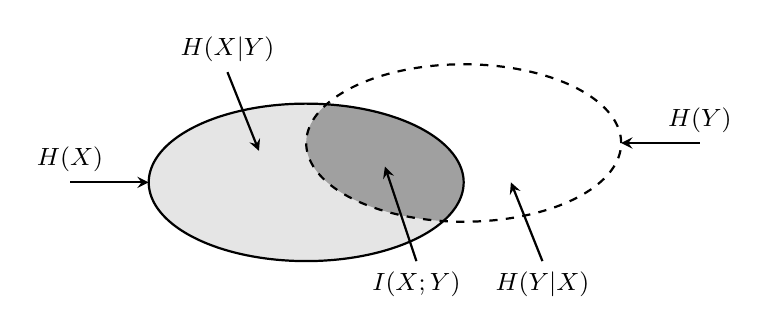
\begin{tikzpicture}[scale=2]
\shorthandoff{>}
% interior H(X) x^2 + 4 y^2 = 1 => y = \pm sqrt(1-x^2)/2
\fill[domain=0:360,samples=200,opacity=.1] plot ({cos(\x)},{.5*sin(\x)});
%
% interior H(Y) (x-1)^2 + 4 (y-1/4)^2 = 1 => y = 1/4 \pm sqrt(1-(x-1)^2)/2
% se cruzan cuando x = 1 \pm sqrt(55)/10 =>
% theta = acos(.5 \pm sqrt(55)/20) para X
% theta = acos(-.5 \pm sqrt(55)/20) para X
\pgfmathsetmacro{\s}{acos(.5-sqrt(55)/20)};
\pgfmathsetmacro{\t}{-acos(.5+sqrt(55)/20)};
\pgfmathsetmacro{\u}{-acos(-.5+sqrt(55)/20)};
\pgfmathsetmacro{\v}{acos(-.5-sqrt(55)/20)-360};
%
% interior I(X;Y)
%\draw[domain=\v:\v] plot ({cos(\x)+1},{.5*sin(\x)+.25}) node{$\bullet$};
\fill[opacity=.3]
   plot [domain=\s:\t,samples=200] ({cos(\x)},{.5*sin(\x)})
-- plot [domain=\u:\v,samples=200] ({cos(\x)+1},{.5*sin(\x)+.25})
-- cycle;
%
% borders H(X) y H(Y)
\draw[domain=0:360,samples=200,thick] plot ({cos(\x)},{.5*sin(\x)});
\draw[dashed,domain=0:360,samples=200,thick] plot ({cos(\x)+1},{.5*sin(\x)+.25});
%
% flechas y flechas condicionales
\draw[thick,>=stealth,<-] (-1,0)--(-1.5,0) node[above]{\small $H(X)$};
\draw[thick,>=stealth,<-] (-.3,.2)--(-.5,.7) node[above]{\small $H(X|Y)$};
%
\draw[thick,>=stealth,<-] (2,.25)--(2.5,.25) node[above]{\small $H(Y)$};
\draw[thick,>=stealth,<-] (1.3,0)--(1.5,-.5) node[below]{\small $H(Y|X)$};
%
\draw[thick,>=stealth,<-] (.5,.1)--(.7,-.5) node[below]{\small $I(X;Y)$};
\end{tikzpicture}